\begin{comment}
Provide context and motivation for your project.
• What existing solutions or research are relevant?
• Why did you choose this topic?
Example: Recent advances in deep learning have enabled effective noise suppression, but many
models are too large for mobile deployment. This project explores efficient architectures suitable
for embedded systems
\end{comment}

\noindent
Despite its relatively recent history, with the first publication of a working draft in only 
2011\footnote{\url{https://www.w3.org/TR/2011/WD-webaudio-20111215/}}, the WebAudio API has seen 
extensive development over the course of a decade, eventually receiving an endorsement from the W3C 
in 2021 as a Recommendation\footnote{\url{https://www.w3.org/TR/webaudio-1.0/}}. Notably, its primary 
\texttt{AudioContext} interface has been fully supported by most major web browsers since at least 
2015\footnote{\url{https://developer.mozilla.org/en-US/docs/Web/API/Web_Audio_API\#browser_compatibility}},
with the only exception being Safari which implemented support in 
2021\footnote{\url{https://developer.apple.com/documentation/safari-release-notes/safari-14_1-release-notes\#WebKit-Framework}}.

Of course, audio has existed for a much longer time than that on the internet. As Boris Smus describes 
in their brief history of audio on the web \cite{boris_smus}, initially that was through the Flash external 
plugin for browsers, and then later through the HTML5 \texttt{<audio>} element which was instead natively 
supported by the web browser itself. In fact, it's this \texttt{<audio>} element that allows music 
streaming websites like Bandcamp to preview an artist's music through the web browser 
(see Fig. \ref{fig:wanderstop}).

\begin{figure}[!htbp]
	\centering
	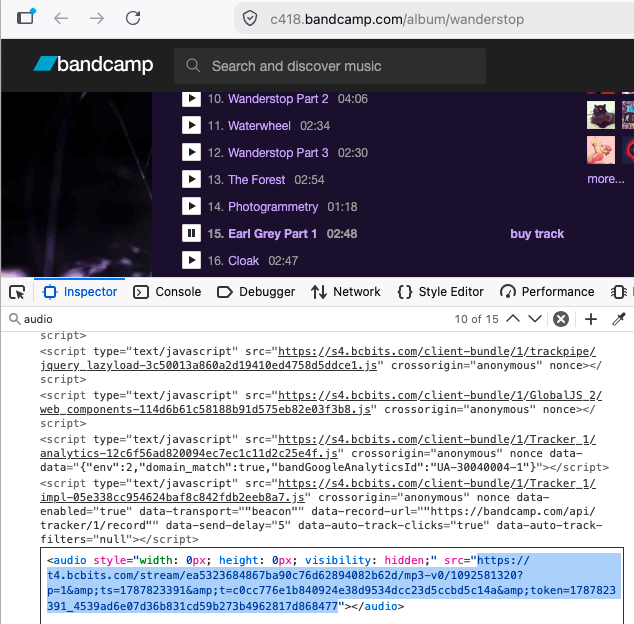
\includegraphics[width=0.6\columnwidth]{images/wanderstop-0}
	
	\texttt{Input ... from `1092581320.mp3' Duration: 00:02:48.00, ..., bitrate: 236 kb/s}

	\caption{Bandcamp allows artists to offer their listeners a compressed and lower bitrate MP3 preview of their tracks, played in the browser through the HTML5 \texttt{<audio>} element. The text above is the result of \texttt{ffprobe 1092581320.mp3}}
	\label{fig:wanderstop}
\end{figure}

But one thing Flash's plugin did for web audio that HTML5's \texttt{<audio>} element doesn't do, is 
allow for interactive audio. For example, a synthesizer/sampler/sequencer like the one this project 
will aim to build, would require a predictable amount of latency between a person pressing a key on 
their keyboard and the corresponding sound being played through their speakers, something that the 
\texttt{<audio>} element just wasn't designed for.

\begin{comment}
Instead, it was designed for cases like Bandcamp's 
song previews, where a one second delay between pressing to pause a song and the song actually pausing,
though annoying, is ultimately benign and would likely be fixed by restarting the browser. But for a real
time instrument like a web synthesizer? That would be incredibly disorientating for a live performance; 
having to wait one second to hear the note they want to play would make the instrument virtually 
unusable.
\end{comment}

That is the kind of problem the WebAudio API attempts to solve, and why it has been possible for 
synthesizers and other real time instruments to be built for the web. For example stevengoldberg's 
emulation of the Juno-106 synthesizer\footnote{\url{https://github.com/stevengoldberg/juno106}} 
built for the web in 2015, to ryukau's collection of 
synthesizers\footnote{\url{https://github.com/ryukau/UhhyouWebSynthesizers}} build for the web which 
use the aforementioned \texttt{AudioContext} interface as the backbone of its audio framework 
(see Fig. \ref{fig:ryukau}).

\begin{figure}[!hbtp]
\begin{minted}{javascript}
// Copyright Takamitsu Endo (ryukau@gmail.com)
// SPDX-License-Identifier: Apache-2.0

export class Audio {
  cachedBuffer = null;
  constructor() {
  	// Initialise AudioContext
    this.audioContext = new AudioContext();
  }
  play() {
    // If no AudioBuffer
    if (!this.cachedBuffer) {
      // Create AudioBuffer object
      let buffer = this.audioContext.createBuffer(
        this.audioContext.sampleRate);
      for (let i = 0; i < this.wave.channels; ++i) {
        // Write to AudioBuffer
        buffer.copyToChannel(new Float32Array(
          this.wave.data[i]), i, 0);
      }
      this.cachedBuffer = buffer;
    }
    // And set AudioContext's AudioBuffer to our's
    this.source = 
      this.audioContext.createBufferSource();
    this.source.buffer = cachedBuffer;

    // And play
    this.source.start();
  }
}
\end{minted}
\caption{Heavily redacted version of the custom Audio class used by ryukau\textsuperscript{6} at 
\texttt{common/wave.js} which uses the WebAudio API}
\label{fig:ryukau}
\end{figure}
